% Biên dịch bằng XeLaTeX hoặc Tectonic.
\documentclass[11pt,a4paper]{article}
\usepackage[left=22mm,right=22mm,top=18mm,bottom=21mm]{geometry}
\usepackage{fontspec}
\setmainfont{texgyretermes}[Extension=.otf,UprightFont=*-regular,
  BoldFont=*-bold,ItalicFont=*-italic,BoldItalicFont=*-bolditalic]
\usepackage{graphicx,tabularx,booktabs,array,enumitem,titlesec,tikz}
\usepackage{hyperref}
\definecolor{ink}{HTML}{244F68}
\hypersetup{unicode,colorlinks=true,urlcolor=ink,linkcolor=ink,
  pdftitle={Xây dựng dữ liệu song song Hán Nôm và Quốc ngữ}}
\graphicspath{{assets/}}
\setlength{\parindent}{0pt}
\setlength{\parskip}{5pt}
\linespread{1.15}
\titleformat{\section}{\Large\bfseries}{\textcolor{ink}{\thesection.}}{.4em}{}
\titleformat{\subsection}{\large\bfseries}{\thesubsection}{.5em}{}
\titlespacing*{\section}{0pt}{12pt}{4pt}
\titlespacing*{\subsection}{0pt}{9pt}{3pt}
\newcolumntype{Y}{>{\raggedright\arraybackslash}X}
\renewcommand{\arraystretch}{1.22}
\setlist[enumerate]{leftmargin=1.65em,itemsep=4pt,topsep=3pt,parsep=0pt}

% Tọa độ khung lấy từ box đầu tiên trong Label.txt, đổi sang hệ trục của ảnh.
\newcommand{\pageexample}[3]{%
  \begin{tikzpicture}
    \node[anchor=south west,inner sep=0] (scan) at (0,0)
      {\includegraphics[height=76mm]{#1}};
    \begin{scope}[x={(scan.south east)},y={(scan.north west)}]
      \draw[draw=ink,line width=.9pt] #2 rectangle #3;
    \end{scope}
  \end{tikzpicture}}
\begin{document}
\begin{center}
{\LARGE\bfseries Xây dựng dữ liệu song song\\ Hán Nôm và Quốc ngữ}
\end{center}

\section{Giới thiệu}
Đồ án xây dựng bộ dữ liệu ghép từng câu hoặc cụm Hán Nôm trên ảnh sách với phần phiên âm hoặc bản dịch Quốc ngữ tương ứng. Mỗi cặp cần giữ đúng nội dung hai vế và có định danh để người đọc tìm lại vùng chữ trên trang gốc.

Phạm vi gồm \textit{Truyện Kiều}, \textit{Ca dao} (digcoll\_14470), \textit{Ca Dao Ngạn Ngư Phương Ngôn} và \textit{Tiên Phả Dịch Lục} (hai tập). Sản phẩm của mỗi sách gồm ảnh trang, nhãn vị trí dòng chữ và bảng căn chỉnh CSV/XLSX.

\section{Dữ liệu và công cụ sử dụng}
\subsection*{Nguồn dữ liệu Truyện Kiều}
\begin{itemize}[leftmargin=1.3em,itemsep=4pt,topsep=3pt,parsep=0pt]
\item \textbf{Bản quét.} Bản Duy Minh Thị 1872 do An Chi phiên âm, chú giải và thảo luận gồm 598 trang PDF. Số trang trong báo cáo tính theo thứ tự của PDF. \href{https://drive.google.com/drive/folders/1Pr7seLVvka4jzIsRtrgNLLtrS88EjP6M?usp=drive_link}{[Thư mục dữ liệu của đề tài]}
\item \textbf{Bản văn đối chiếu.} Tệp \texttt{TruyenKieu.txt} lấy từ bản Nôm và Quốc ngữ trên Wikisource. Tệp giữ số dòng gốc và ghi chú để tra lại những chỗ khuyết hoặc lệch số. Khi hai bản khác chữ, người duyệt đối chiếu với ảnh của bản quét. \href{https://vi.wikisource.org/wiki/Truy%E1%BB%87n_Ki%E1%BB%81u_%28b%E1%BA%A3n_Duy_Minh_Th%E1%BB%8B_1872%29}{[Wikisource tiếng Việt, \textit{Truyện Kiều} (bản Duy Minh Thị 1872)]}
\end{itemize}

\subsection*{Công cụ theo công đoạn}
\begin{tabularx}{\linewidth}{@{}p{.38\linewidth}Y@{}}
\toprule
\textbf{Công cụ} & \textbf{Vai trò trong hệ thống}\\ \midrule
PyMuPDF, Pillow & Dựng ảnh từ PDF và trích vùng chữ để kiểm tra.\\
Kim Hán Nôm, VietOCR & Nhận dạng lần lượt chữ Hán Nôm và Quốc ngữ. VietOCR chạy qua ONNX Runtime trên CPU.\\
React, TypeScript & Hiển thị ảnh, sửa khung dòng, căn chỉnh và duyệt từng vị trí chưa khớp.\\
FastAPI, SQLite, openpyxl & Lưu liên kết giữa ảnh và câu, ghi quyết định duyệt và xuất bảng XLSX có màu đánh dấu.\\
\href{https://nomnaviet.com/en/search}{Nôm Na Việt} & Tra chữ theo âm Quốc ngữ, xem nghĩa và so sánh dị thể khi duyệt.\\
\bottomrule
\end{tabularx}

\newpage
\section{Quy trình thực hiện}
\subsection*{Từ ảnh trang đến cặp câu}
\begin{enumerate}
\item \textbf{Xác định trang và chiều đọc.} Phân loại trang Nôm, Quốc ngữ và phần phụ. Với \textit{Truyện Kiều}, liên kết trang chữ Nôm với trang phiên âm tương ứng.
\item \textbf{Nhận dạng và sửa dòng.} Chạy OCR trên vùng cần đọc hoặc nạp ảnh và nhãn có sẵn từ \texttt{Label.txt}. Đối chiếu với ảnh để sửa chữ, thứ tự đọc và bốn điểm bao quanh mỗi dòng.
\item \textbf{Căn chỉnh theo nội dung.} Ghép dòng Nôm với câu Quốc ngữ cùng ý. Khi một câu trải qua nhiều dòng, người làm có thể tách hoặc gộp cặp và giữ liên kết với từng vùng ảnh.
\end{enumerate}

\subsection*{Trang Duyệt nhanh}
Sau khi chọn sách và bấm \textbf{Quét đối chiếu}, người duyệt xem các vị trí còn cần quyết định. Với \textit{Truyện Kiều}, hệ thống tìm dòng tham chiếu bằng nội dung của cả hai vế. Khi số chữ lệch hoặc chưa xác định được dòng tương ứng, thẻ hiển thị cả dòng để đọc trong ngữ cảnh.

\begin{tabularx}{\linewidth}{@{}p{.26\linewidth}Y@{}}
\toprule
\textbf{Trên thẻ duyệt} & \textbf{Cách xử lý}\\ \midrule
Ảnh hai trang & Mở vùng chữ, cả dòng hoặc cả trang. Khung nét đứt biểu thị vị trí chữ ước lượng trong khung dòng.\\
Chữ và âm đọc & So chữ trên ảnh với gợi ý từ Nôm Na Việt, xem dị thể hoặc sửa Quốc ngữ. Có thể mở màn hình căn chỉnh để kiểm tra lại cặp.\\
Quyết định & Chọn \textbf{Đúng · đen} khi hai vế tương ứng, \textbf{Đỏ} khi khác, hoặc \textbf{Thiếu từ điển} khi chưa tra được chữ (xuất màu đỏ). Chọn \textbf{Để sau} nếu cần xem lại.\\
\bottomrule
\end{tabularx}

\textbf{Ví dụ cần xem bản quét.} Ở câu thứ hai của trang Nôm 046, tệp TXT ghi “cợt nhau”. Ảnh trang Quốc ngữ 047 dưới đây cho thấy An Chi phiên âm là “ghét nhau”. Bảng xuất giữ cách đọc trên ảnh. Quyết định trên thẻ được lưu ngay và có thể hoàn tác.

\begin{center}
\begin{tikzpicture}
  % Cắt vùng chứa dòng thứ hai ở độ rộng 100 mm cho toàn ảnh gốc.
  \clip (20mm,110mm) rectangle (73mm,117.7mm);
  \node[anchor=south west,inner sep=0] at (0,0)
    {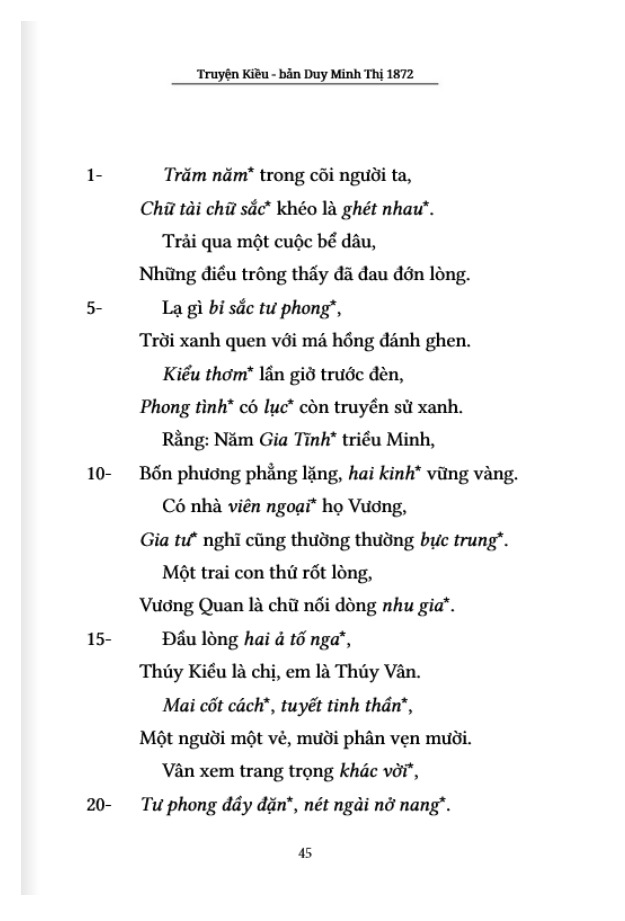
\includegraphics[width=100mm]{kieu-047.jpg}};
\end{tikzpicture}
\end{center}

\subsection*{Xác nhận và xuất dữ liệu}
Sau khi xác nhận cặp, hệ thống chuẩn hóa hai vế, loại dấu câu và khoảng trắng dư, rồi xuất các cặp đủ nội dung. Mỗi dòng CSV/XLSX lưu tên ảnh, định danh câu, chữ Nôm và Quốc ngữ. Nhãn vùng chữ đi kèm ảnh để có thể kiểm tra lại từng dòng.

\newpage
\section{Kết quả đạt được}
\subsection*{Truyện Kiều (bản Duy Minh Thị 1872)}
Gói kết quả gồm PDF nguồn, ảnh theo loại trang, nhãn OCR theo định dạng PPOCRLabel (\texttt{Label.txt}, \texttt{fileState.txt}) và hai bảng căn chỉnh CSV, XLSX.

\begin{tabularx}{\linewidth}{@{}Yr@{}}
\toprule
\textbf{Thành phần trong gói xuất} & \textbf{Khối lượng}\\ \midrule
Ảnh trang thơ có nhãn & 163 trang Nôm và 163 trang Quốc ngữ\\
Vùng dòng trong nhãn OCR & 3.259 vùng Nôm và 3.259 vùng Quốc ngữ\\
Cặp Nôm -- Quốc ngữ trong mỗi bảng & 3.259 cặp\\
\bottomrule
\end{tabularx}

\begin{center}
\begin{tabular}{@{}c@{\hspace{12mm}}c@{}}
\pageexample{kieu-046.jpg}{(.741,.593)}{(.792,.841)} &
\pageexample{kieu-047.jpg}{(.251,.794)}{(.664,.823)}\\
{\small Trang 046 · Chữ Nôm} & {\small Trang 047 · Quốc ngữ}
\end{tabular}\\[4pt]
{\small\textbf{Hình 1.} Hai khung đánh dấu câu đầu theo tọa độ trong nhãn OCR.\\
Cặp có định danh kết thúc bằng \texttt{.046.1}, với vế Quốc ngữ “trăm năm trong cõi người ta”.}
\end{center}

\section{Đánh giá và thảo luận}
Đối chiếu cả bốn cột cho thấy CSV và XLSX khớp đủ 3.259 cặp, mỗi cặp có một định danh riêng. Theo tiêu chí màu của đề tài, 61 trong 22.805 chữ Nôm được tô đỏ, tương ứng độ tương đồng \textbf{99,73\%} (ngưỡng yêu cầu 95\%). Chỉ số này đo mức tương ứng đã đánh dấu sau hiệu chỉnh. Khác biệt giữa các bản phiên âm vẫn cần đọc lại trên ảnh.

\section{Kết luận và hướng phát triển}
Đã hoàn thành bộ dữ liệu \textit{Truyện Kiều} và trang Duyệt nhanh để đối chiếu từng chữ với ảnh và từ điển. Bước tiếp theo là áp dụng quy trình cho ba tài liệu còn lại và rà soát các chữ còn đánh dấu đỏ.

\newpage
\section*{Kết quả theo tài liệu \normalfont\large (bổ sung cho mục 4)}
% Điền kết quả từng sách vào các khoảng dưới đây khi có dữ liệu.
\subsection*{Ca dao (digcoll\_14470)}
\vfill
\subsection*{Ca Dao Ngạn Ngư Phương Ngôn}
\vfill
\subsection*{Tiên Phả Dịch Lục (hai tập)}
\vspace*{\fill}
\end{document}
